\documentclass[a4paper, 12pt]{article}

\usepackage[UTF8]{ctex}
\usepackage{graphicx}
\usepackage{float}
\usepackage{hyperref}

\graphicspath{{images/}}

\hypersetup{hidelinks}

\title{数字逻辑设计大作业设计报告\\基于 FPGA 的附棋钟国际象棋}
\author{王殊凡\ \ 姚秉辰}
\date{\today}

\begin{document}
    \maketitle
    \thispagestyle{empty}

    \newpage
    \pagenumbering{roman}
    \tableofcontents

    \newpage
    \pagenumbering{arabic}

    \section{设计说明}

        我们的大作业是基于 FPGA 设计的「附棋钟国际象棋」。

        我们使用的设备有:Xilinx Kintex-7 FPGA(开关、按钮、LED、七段数码管、蜂鸣器),PS/2 接口键盘,VGA 输出显示器。

        该时序电路实现的主要功能有:

        \begin{itemize}
            \item 通过 SWORD 板上开关和按钮打开电源、复位游戏。

            \item 通过键盘控制棋子,以实现国际象棋的所有操作。

            \item 通过 SWORD 板上开关和按钮的操作控制棋钟,以实现棋钟的设置时间、交替计时、暂停、宣告时间耗尽等功能。
            
            \item 通过显示器显示棋盘画面,以供玩家查看当前局面。
        \end{itemize}

        该时序电路旨在通过电子方式复刻现实中的国际象棋游戏,以提供不依赖于实际棋盘和棋钟设备的游戏方式。因此其功能与基于实际棋盘和棋钟的情况无异,即只提供了基本的棋盘和棋钟操作,操作是否符合规则与胜负判断仍需要裁判介入或棋手自行处理。我们相信这样的处理有利于习惯传统国际象棋下棋方式的棋手、裁判与赛会组织更好适应我们的电子替代方案。

        我们相信这一设计能够在当下帮助人们规避昂贵的棋盘与棋钟设备,有助于国际象棋的推广和发展。同时这一设备也为国际象棋赛事,在未来通过大屏转播比赛等方面作出了有益的探索。

    \section{核心模块说明与仿真}

        下图是电路的分层设计结构。
        
        \begin{figure}[H]
            \centering
            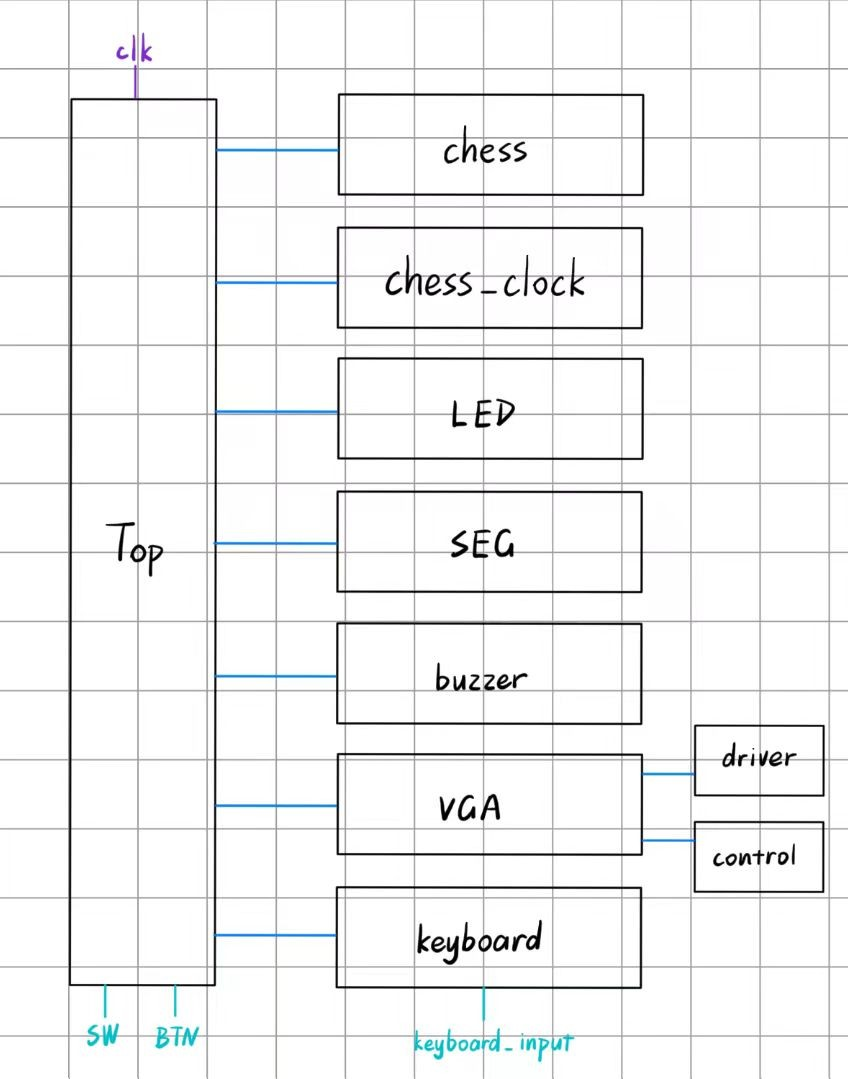
\includegraphics[width=0.6\textwidth]{hierarchical_design.jpg}
            \caption{分层设计}
        \end{figure}

        可以看到,顶层模块 \texttt{Top} 输入来自 FPGA 的时钟信号 clk、开关信号 SW 和按钮信号 BTN。在顶层模块 \texttt{Top} 下,主要有 7 个子模块:\texttt{chess}、\texttt{chess\_clock}、\texttt{LED}、\texttt{SEG}、\texttt{buzzer}、\texttt{VGA}、\texttt{key}。

        下图是电路的状态机图。

        \begin{figure}[H]
            \centering
            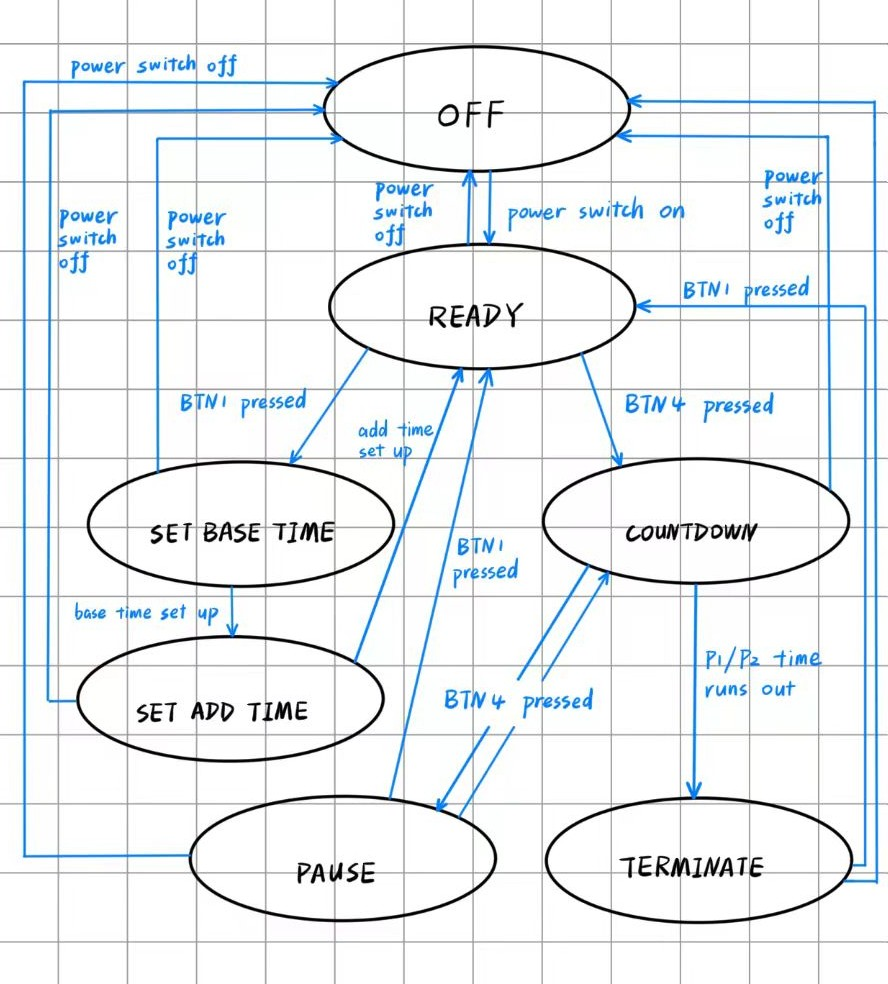
\includegraphics[width=0.6\textwidth]{statemachine_chart.jpg}
            \caption{状态机图}
        \end{figure}

        电路的状态及转移主要基于棋钟设计,其细节我们将在对应的子模块处详细叙述。

        下面我们将依次介绍子模块。

        \subsection{\texttt{chess} 模块}

            \texttt{chess} 模块用于实现国际象棋的控制逻辑。其记录了国际象棋中各个棋子的位置和存活情况,并可以模拟棋盘光标移动、棋子选择与移动的基本操作。具体地,其通过按键输入控制光标位置并选择棋子,支持将选中的棋子移动到目标位置,并自动清除目标位置上的其他棋子。

            \texttt{chess} 模块输入时钟信号 clk、使能信号 start、复位信号 rst 和键盘信号 key,输出光标位置 crt,以及各棋子的状态信号 wp0-wk、bp0-bk。

            当 rst 信号有效时:光标与所有棋子被初始化为其标准起始位置。在 start 信号有效时:根据 key[4:1] 的上升沿检测,控制光标的上下左右移动;根据 key[0] 的上升沿检测进行确认操作,若未选中任何棋子,则调用 select\_piece 函数查找当前位置是否有棋子,并标记为选中。若已有选中棋子,则调用 move\_piece 函数将其移动到当前光标位置,并取消选中状态。如果目标位置上有其他棋子,则自动清除该棋子。

            \begin{figure}[H]
                \centering
                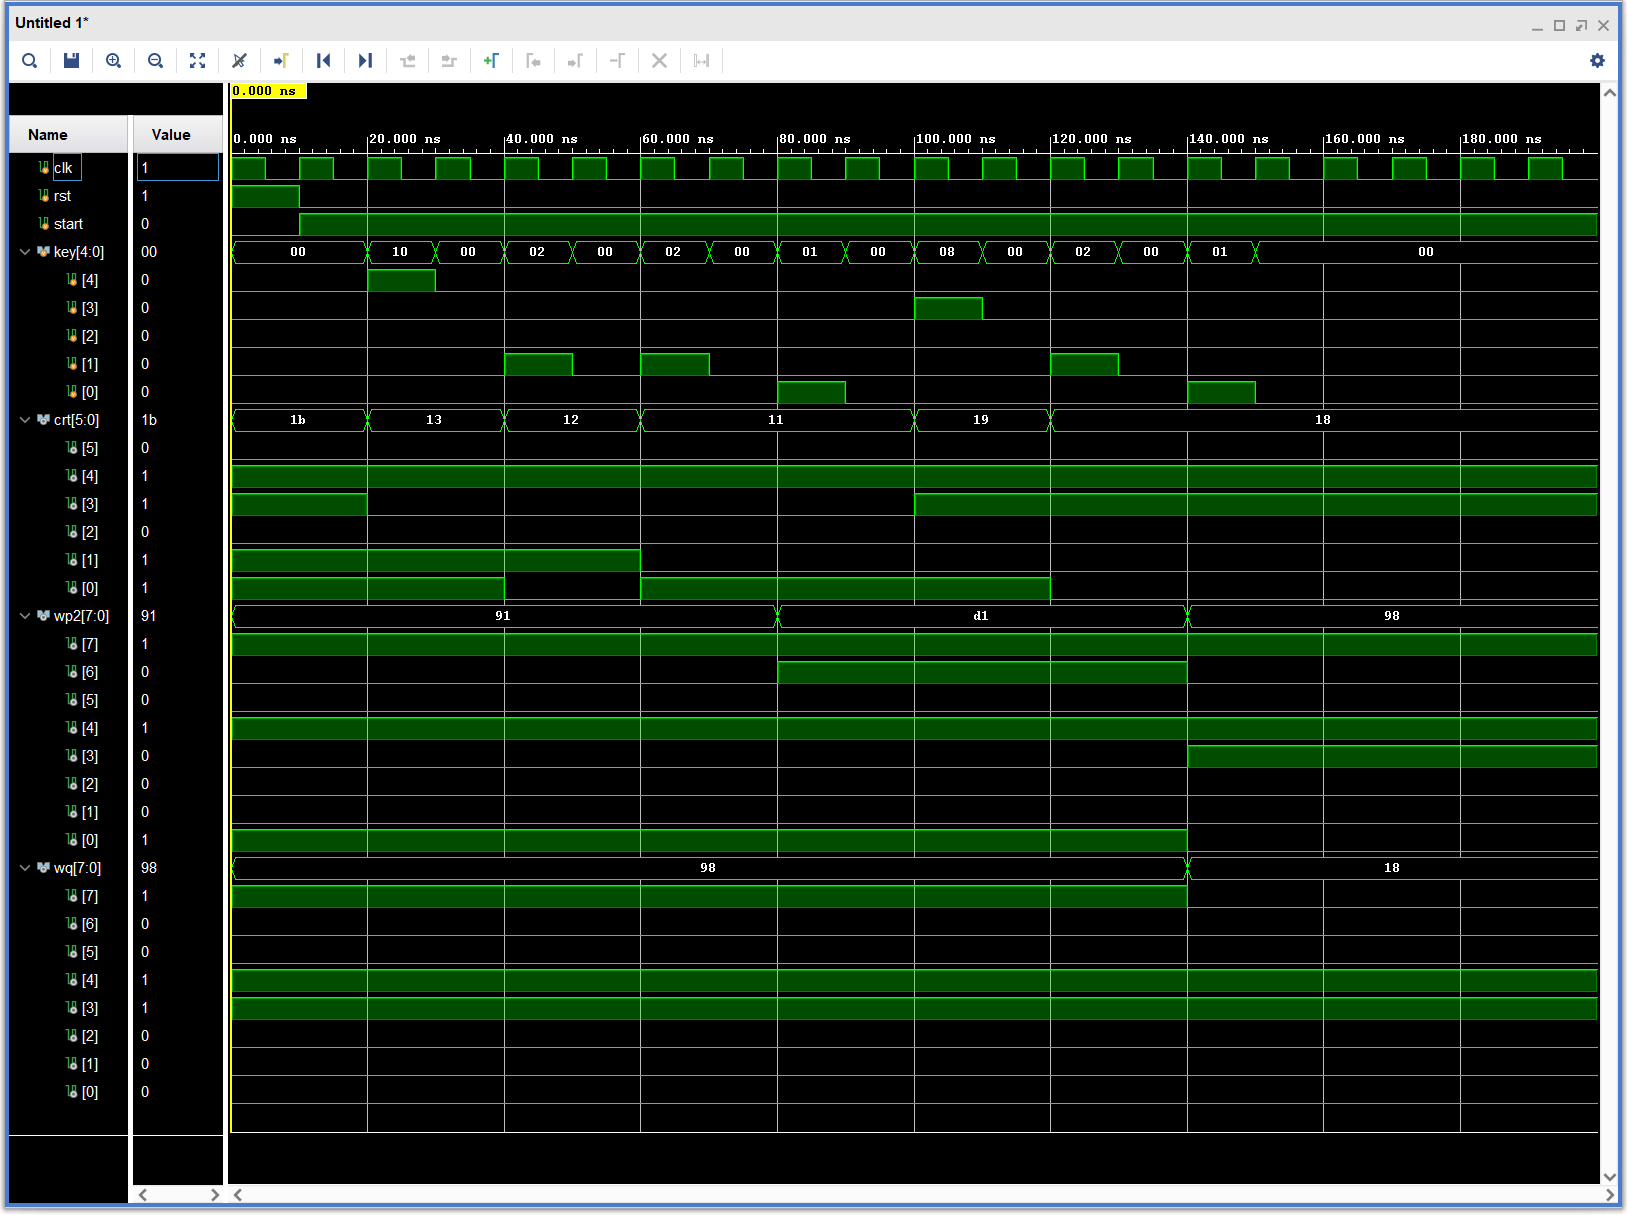
\includegraphics[width=0.6\textwidth]{wave0}
                \caption{\texttt{chess} 模块仿真波形}
            \end{figure}

            可以看到,在仿真波形中,随着键盘 key 依次发出左、下、下信号,光标位置 crt 由初始的 d4 格移动到 c2 格。在键盘 key 发出 enter 信号后,位于 c2 格的兵 wp2[6] 变为 1,表明该子被选中。随后键盘 key 依次发出右、下信号,光标位置 crt 由 c2 格移动到 d1 格。在键盘 key 发出 enter 信号后,位于 d1 格的后 wq[7] 变为 0,表明该子被移出棋盘,同时兵 wp2 的坐标由 c2 格移动到 d1 格。

            值得说明的是,使能信号 start 仅在 COUNTDOWN 状态下为高电平,也即 \texttt{chess} 模块仅在该状态下可用。
        
        \subsection{\texttt{chess\_clock} 模块}

            \texttt{chess} 模块用于实现棋钟的控制逻辑。其通过按键和开关控制玩家切换、时间调整与启动倒计时,同时通过七段数码管显示当前时间,并在比赛结束时驱动蜂鸣器指示。同时其可以在倒计时、暂停与终止状态之间切换,以满足国际象棋正规比赛的需要。

            \texttt{chess} 模块输入时钟信号 clk、电源开关信号 power\_switch、玩家切换信号 toggle\_switch、按钮信号 btn、用于闪烁提示的 0.5秒周期时钟信号 clk\_500ms、用于倒计时的 1 秒周期时钟信号 clk\_1s,输出七段数码管数据 hex、小数点数据 point、数码管使能信号 LEs、蜂鸣器使能信号 buzzer\_en、当前状态信号 state。

            起始时棋钟处于 OFF 状态,当 power\_switch 为高电平时,进入 READY 状态,七段管与屏幕亮起。默认基础时间(basic time)为 15 分钟,每步加时(increment)为 10 秒。按下 btn1 进入 SET BASE TIME 状态,此时可通过 btn2 和 btn3 增减基础时间的分或秒,btn1 控制编辑位置。编辑完成后再次按 btn1 进入 SET ADD TIME 状态,此时可通过 btn2 和 btn3 增减每步加时的分或秒,btn1 控制编辑位置。编辑完成后再次按 btn1 回到 READY 状态。按下 btn4 进入 COUNTDOWN 状态,启动倒计时并持续更新当前玩家剩余时间。当前玩家时间每秒钟递减 1 秒,按下切换开关可切换玩家并增加加时。在 COUNTDOWN 状态下按 btn4 可进入 PAUSE 状态暂停计时,再次按下恢复倒计时。当任意玩家时间归零,进入 TERMINATE 状态,蜂鸣器开始闪烁发声,再次按 btn1 回到 READY 状态完成复位。在除 OFF 状态外的任意状态中,只要 power\_switch 为低电平,则进入 OFF 状态,此时七段管与屏幕均熄灭。

            \begin{figure}[H]
                \centering
                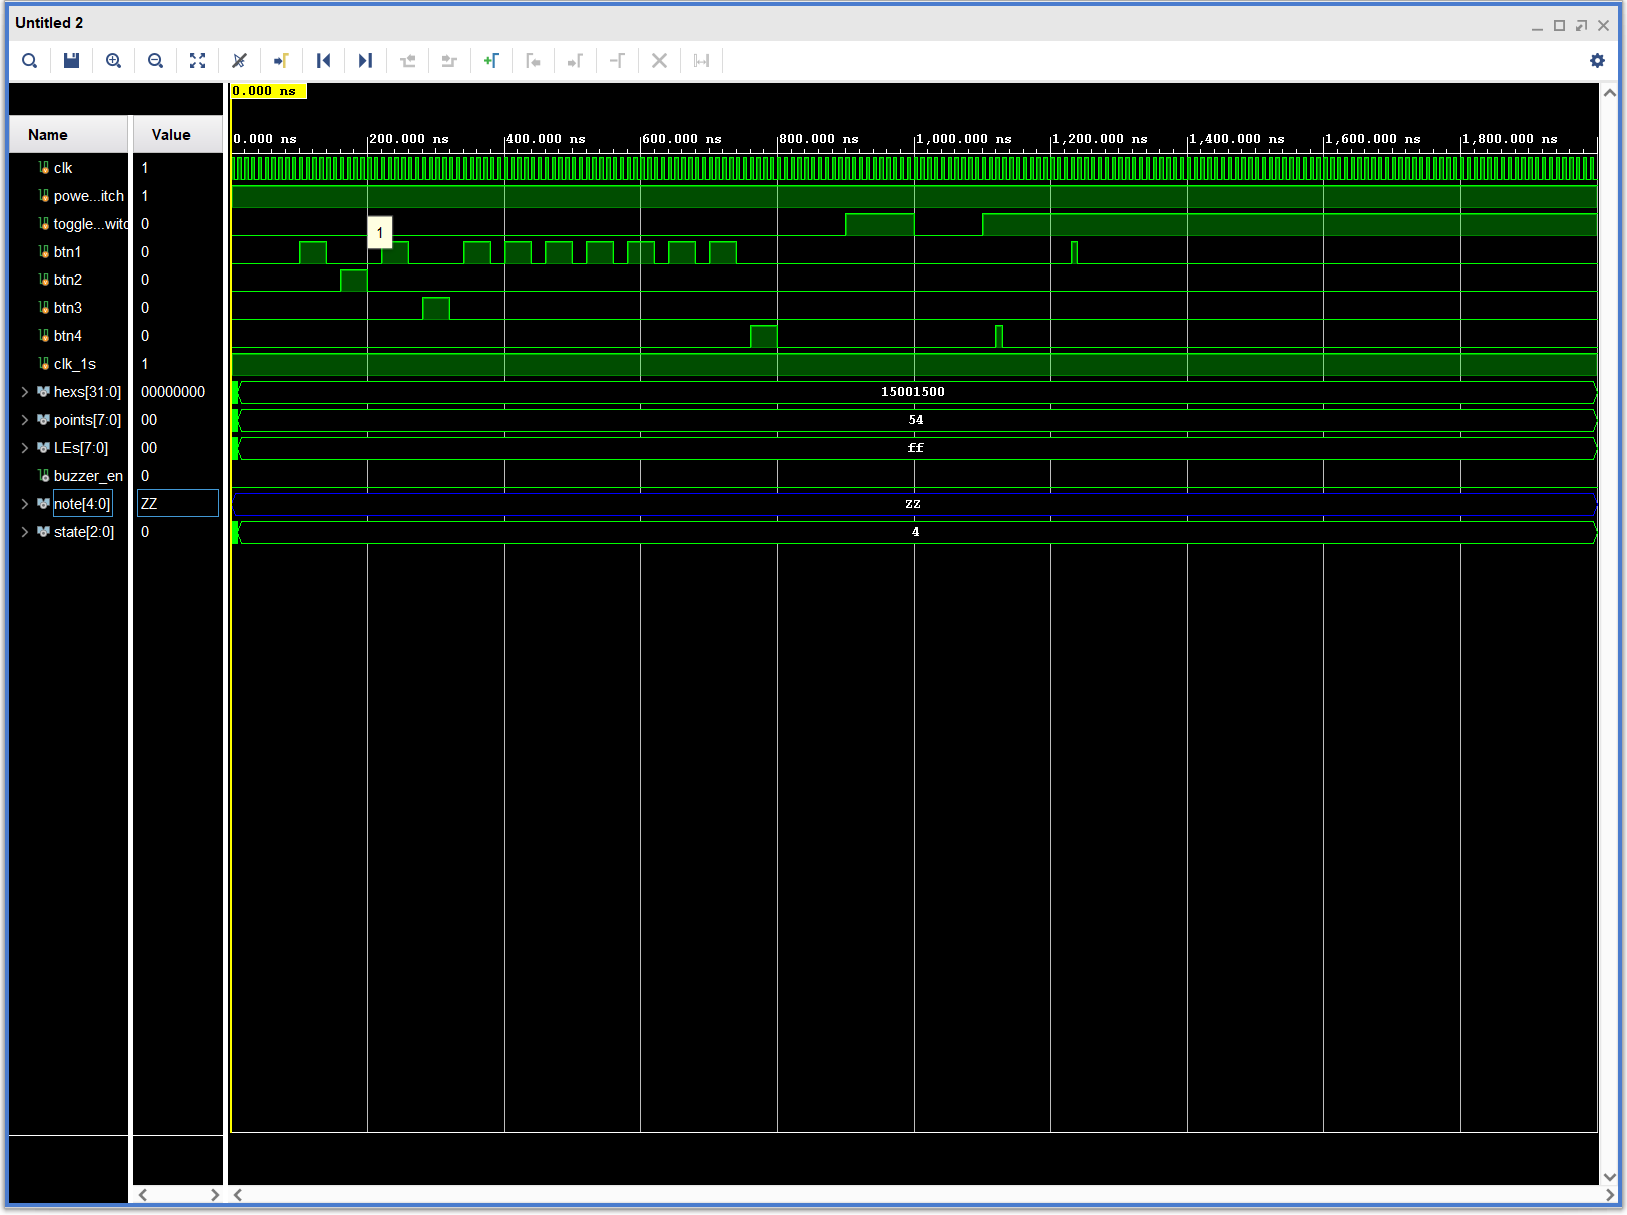
\includegraphics[width=0.6\textwidth]{wave1}
                \caption{\texttt{chess\_clock} 模块仿真波形}
            \end{figure}

            可以看到仿真波形的结果与前文中的预期运行过程一致。
        
        \subsection{\texttt{LED} 模块}

            \texttt{LED} 模块沿用了学期内 Lab 的设计,故不再详细叙述。

        \subsection{\texttt{SEG} 模块}

            \texttt{SEG} 模块沿用了学期内 Lab 的设计,故不再详细叙述。

        \subsection{\texttt{buzzer} 模块}

            \texttt{buzzer} 模块实现了一个蜂鸣器音调控制器,可根据输入的音符编号生成对应频率的方波信号,用于驱动蜂鸣器发声。并通过使能信号控制是否启用蜂鸣器输出。

            \texttt{buzzer} 模块输入时钟信号 clk、使能信号 EN、音符编号 note,输出蜂鸣器方波信号 beep。

        \subsection{\texttt{VGA} 模块}

            \texttt{VGA} 模块下有两个子模块 \texttt{VGA\_driver} 和 \texttt{VGA\_ctrl}。前者是 VGA 驱动模块,用于生成 VGA 所需的水平与垂直扫描计数器,判断当前扫描点是否处于有效显示区域,将图象控制模块提供的像素色彩数据转换为 RGB 信号输出,并同时输出 VGA 的水平和垂直同步信号。后者是图像控制模块,根据 \texttt{chess} 模块提供的国际象棋盘面信息和当前扫描点坐标决定应显示的内容,并从 ROM 中读取棋盘背景、棋子、光标、选中框等图形数据,输出扫描点的像素色彩数据。

            \texttt{chess} 模块输入时钟信号 clk、复位信号 rst、使能开关 switch、光标位置 crt,以及各棋子的状态信号 wp0-wk、bp0-bk,输出 RGB 颜色信号 vga\_red、vga\_green、vga\_blue、VGA 同步信号 vga\_hs、vga\_vs。

        \subsection{\texttt{key} 模块}

            \texttt{key} 模块实现 PS/2 键盘输入采集功能。

            这一部分我们借鉴了潘致远学长在浙江大学 2019-2020 秋冬学期数字逻辑设计课程设计 \footnote{\href{https://github.com/pan2013e/FPGA-Jack-Frost}{https://github.com/pan2013e/FPGA-Jack-Frost}} 的代码,并在此基础上进行了修改以符合本设计需求。

    \section{调试过程分析}

        在项目初始阶段,我们采用 coe 文件与 Xilinx IP 核协同工作的方式实现图像像素化与数据录入。然而,该方法在实践过程中存在显著的工程复杂性。经技术评估后,我们开发了基于 Python 的自动化处理流程,直接将 png 格式图像转化为 mem 二进制文件,大幅简化了图像数据导入流程,最终确立 mem 文件作为系统标准图像存储方案。

        在 VGA 显示调试阶段,国际象棋棋子的非规则几何形状与MEM文件的矩形像素矩阵特性产生兼容性问题。传统解决方案需引入 Alpha 通道实现透明效果,但受限于已完成的 VGA 扫描架构,该模块仅支持 RGB 三通道 24 位色深。通过色彩空间分析,我们发现棋盘设计中完全规避了正红色(12'hF00)的使用,因此创新性地将图像无效像素统一替换为正红色值,并在渲染管线中设置色彩过滤逻辑:当检测到正红色像素时自动跳过渲染。该方案在保证显示效果的同时,有效规避了架构修改带来的重新设计风险。

        在棋钟模块开发过程中,LED 数字显示稳定性成为技术瓶颈。由于驱动代码复杂度高、状态机嵌套层级深,传统调试手段收效甚微。项目负责人通过长达 14 小时的连续技术攻关,采用信号分段捕获与时序回溯分析法,最终在凌晨三点成功定位到时序冲突,通过优化时钟域同步机制彻底解决了操作无效问题。该突破性进展为系统实时性提供了关键保障。

    \section{小组主要工作说明}

        本项目的设计与实现完全由小组成员独立完成,从选题构思、方案设计到系统实现均体现了原创性,没有任何参考工程。在项目初期,我们自主完成了国际象棋规则引擎的核心算法设计,包括棋子移动逻辑、棋盘状态管理和胜负判定机制;在硬件实现层面,我们独立开发了 FPGA 上的多模块协同架构,包括 VGA 显示控制器、棋钟状态机和键盘交互系统等关键组件。整个开发过程中,我们仅参考了少量开源代码片段用于 PS/2 键盘协议的实现,并对其进行了深度适配改造以满足特定交互需求。通过自主设计的 Python 图像处理流水线、创新的透明像素替代方案以及历时数十小时的硬件调试攻关,最终实现了具有完整国际象棋规则支持、实时棋钟计时和高质量图形显示的综合性系统。
        
        这项工作的核心价值在于构建了完全自主知识产权的 FPGA 棋类游戏平台,其模块化架构为传统棋类运动的电子化转型提供了可复用的技术范式,所开发的实时渲染优化方案和交互设计原则对嵌入式图形系统开发具有普适性参考意义。

    \section{成员贡献比例}

        \begin{itemize}
            \item 王殊凡:51\%
            \item 姚秉辰:49\%
        \end{itemize}

        小组成员签名:

        \begin{figure}[H]
            \centering
            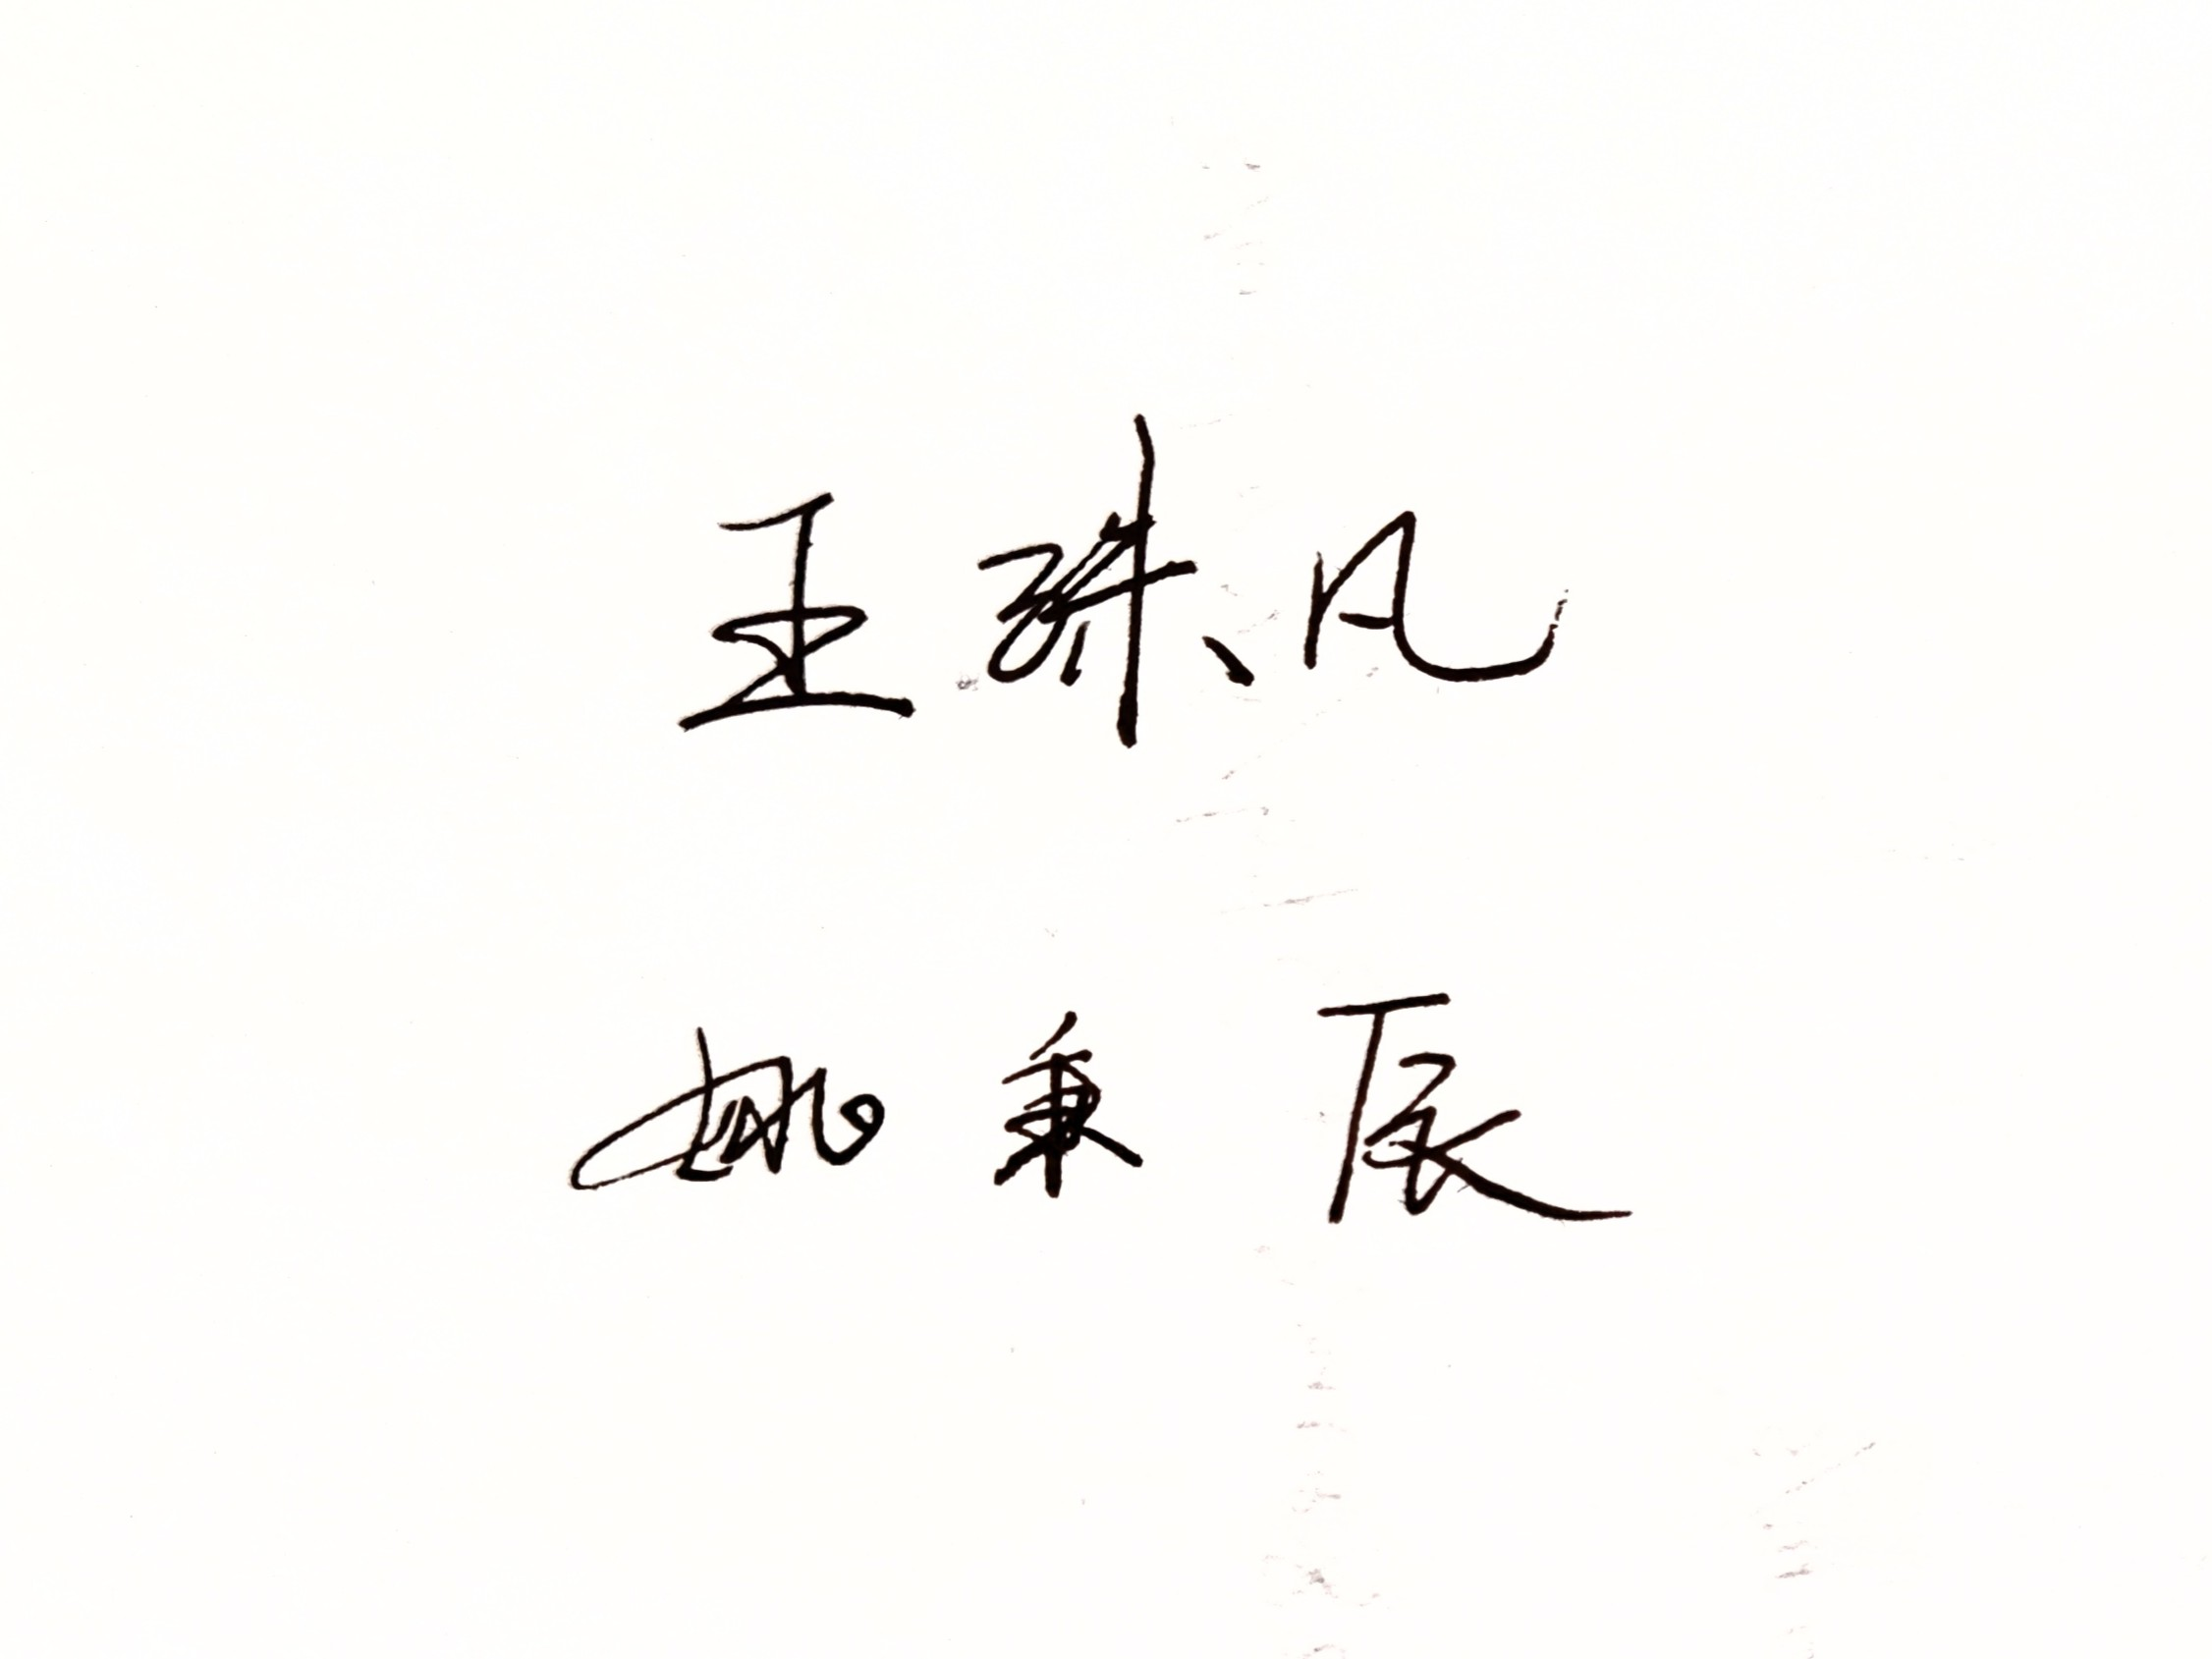
\includegraphics[width=0.6\textwidth]{signature}
            \caption{小组成员签名}
        \end{figure}

    \section{附言}

        本项目的代码已开源,可以通过链接 \href{https://github.com/VictorWang712/FPGA-clock-attached-chess}{\textsf{https://github.com/VictorWang71\\2/FPGA-clock-attached-chess}} 访问。

        本项目的演示视频已发布至哔哩哔哩,可以通过链接 \href{https://www.bilibili.com/video/BV14Q7QznE1D}{\textsf{https://www.bilib\\ili.com/video/BV14Q7QznE1D}} 访问。

\end{document}